% Build: pdflatex main, bibtex main, pdflatex main (twice)
\documentclass[conference]{IEEEtran}

\usepackage{cite}
\usepackage{amsmath,amssymb}
\usepackage{graphicx}
\usepackage{booktabs}
\usepackage{array}
\usepackage{xcolor}
\usepackage{algorithm}
\usepackage{algpseudocode}
\usepackage{tikz}
\usepackage{pgfplots}
\pgfplotsset{compat=1.18}
\usetikzlibrary{positioning,arrows.meta}
\usepackage{url}

\newcommand{\todo}[1]{\textcolor{red}{[TODO: #1]}}
\newcommand{\tool}{OptiNPU}
\newcommand{\ms}{\,\text{ms}}

\begin{document}

\title{Measure, Don't Predict: Accuracy-Guarded Latency\\Optimization of Object Detectors on a Client NPU}

\author{\IEEEauthorblockN{Julien Beloin}
\IEEEauthorblockA{Independent researcher\\
\url{https://github.com/Zeta-12/OptiNPU}}}

\maketitle

\begin{abstract}
Laptops now ship with neural processing units (NPUs) that promise low-power inference, yet modern object detectors run poorly on them. On an Intel Core Ultra NPU, none of seven state-of-the-art real-time detectors runs fastest on the NPU alone, FLOPs do not predict latency, the vendor's per-operation counters overlap, and the compiler can silently cost up to 4.6~AP or hang the device. We present \tool{}, an open-source tool that profiles, validates and optimizes a model for the NPU using on-device measurements only. It rests on an observation that we verify: latency does not depend on the values of dense weights, so any variant of a model, such as a bypassed region, a rewritten operation, or an architecture not yet retrained, can be timed with any weights, before it is trained or calibrated. \tool{} (i)~attributes latency by bypassing module regions in paired, randomized rounds, repeated until a 95\,\% confidence interval is narrow; (ii)~guards accuracy at the task level, with detection agreement and a paired non-inferiority test on COCO AP, repeated on held-out images for approximations; and (iii)~greedily applies exact and approximate rewrites, including a latency-guided mixed-precision search, and reports retraining rewrites with their measured latency. On five models, a repeated measurement always picks the best intervention, while acting on vendor counters, on an additive cost model, or on a regressor fitted to the other models' measurements loses on average 31\,\%, 60\,\% and 21\,\% of the best saving. The optimizer makes YOLO26-N 2.84$\times$ and YOLO26-S 2.02$\times$ faster on the NPU, repairing a silent 4.6-AP loss and a device hang, with AP within 0.1~points of CPU FP32. The held-out confirmation rejects a ResNet-50 mix that loses 0.64~points on the report images, but also three candidates whose mean loss stays within the budget: on the NPU, a single INT8 deployment remains (RF-DETR-N, 1.02$\times$), and two DETR repairs cost latency. NNCF's accuracy-aware quantization, which validates on the CPU, accepts losses our test cannot certify, and two of its six models lose 1.5 and 18 points on the NPU. Optimized the same way, the iGPU is faster on seven of the ten models, but the NPU deployment uses 1.2 to 2.3$\times$ less energy per inference on nine of them.
\end{abstract}

\begin{IEEEkeywords}
neural processing unit, object detection, latency profiling, quantization, mixed precision, compiler validation
\end{IEEEkeywords}

% =====================================================================================================
\section{Introduction}

Client processors now integrate a neural processing unit (NPU) next to the CPU and the integrated GPU (iGPU): Intel Core Ultra, AMD Ryzen AI, Qualcomm Snapdragon~X. Their purpose is to run sustained inference at low power and to leave the CPU and GPU free for the user. Real-time object detection is a natural workload for them, and the detectors of the last two years, mostly descendants of DETR~\cite{carion2020detr} (RT-DETR~\cite{zhao2024rtdetr,lv2024rtdetrv2}, D-FINE~\cite{peng2025dfine}, DEIM~\cite{huang2025deim,huang2025deimv2}, RF-DETR~\cite{robinson2026rfdetr}, YOLO26~\cite{jocher2026yolo26}) reach 40 to 53 COCO AP~\cite{lin2014coco} at a few GFLOPs.

Deploying these detectors on an NPU is nevertheless a trial-and-error exercise. Our measurements on an Intel NPU~3720 (Section~\ref{sec:motivation}) show that:
\begin{itemize}
\item none of seven detectors is fastest on the NPU alone: they run 1.4 to 3.6$\times$ slower than on the iGPU or in a hybrid NPU+iGPU placement;
\item FLOPs do not predict latency: YOLO26-N (5.4~GFLOPs) takes 26.6\ms{}, ResNet-50 at 224~px (8.2~GFLOPs) 3.9\ms{};
\item the vendor's per-operation counters overlap, so their sum is several times the real latency;
\item the compiler fails silently: in its default two-tile mode, YOLO26-N loses 4.6~AP, RT-DETRv2 3.8~AP, and YOLO26-S hangs the device after a few images.
\end{itemize}

Existing tools predict rather than measure. Latency predictors learn per-kernel costs and add them up~\cite{zhang2021nnmeter,li2021hwnasbench,dudziak2020brpnas}. Hardware-aware search and compression use such predictors or lookup tables~\cite{yang2018netadapt,cai2019proxylessnas,tan2019mnasnet,he2018amc}. Mixed-precision methods model the latency of a configuration as the sum of per-layer costs~\cite{yao2021hawqv3}. On this NPU, none of these assumptions holds: costs are not additive, and the compiled graph may be wrong.

We take the opposite approach: \emph{measure, don't predict}. One property of the NPU makes this affordable: \textbf{latency does not depend on the values of dense weights}. A variant of a model can therefore be timed with any weights, before it is trained, calibrated or even designed in PyTorch; only data-dependent operations and weight sparsity need care. We build \tool{} on this property. Our contributions are:
\begin{enumerate}
\item a characterization of a client NPU that explains why prediction fails there: non-additive costs, overlapping counters, value-dependent operations, exploited weight sparsity, and silent compiler errors (Sections~\ref{sec:motivation} and~\ref{sec:premise});
\item a measured profiler, based on region bypassing and paired, randomized, adaptive rounds, which picks better interventions than vendor counters, an additive cost model and a learned regressor on 150 interventions over five models (Section~\ref{sec:eval-profiler});
\item a task-level accuracy guard that combines detection agreement and a paired non-inferiority test on AP, calibrated on real compiler failures, and confirms approximations on held-out images (Section~\ref{sec:guard});
\item a three-tier optimizer (exact, approximate, retraining), with a latency-guided mixed-precision search that does not assume additive costs, evaluated on seven detectors and three image classifiers, against NNCF's accuracy-aware quantization and against the iGPU optimized the same way (Sections~\ref{sec:optimizer} and~\ref{sec:eval-optimizer} to~\ref{sec:eval-igpu});
\item an open-source implementation (Apache-2.0) at \url{https://github.com/Zeta-12/OptiNPU}, which runs every compilation and inference in a watched child process.
\end{enumerate}

% =====================================================================================================
\section{Background and Motivation}
\label{sec:motivation}

\subsection{The Intel NPU 3720}

The NPU of the Intel Core Ultra~5 235U has two neural compute tiles. Each tile has DPU arrays, which run convolutions and matrix products, SHAVE DSP cores, which run the other operations, and DMA engines. OpenVINO~\cite{openvino} compiles a whole graph for it, given in its intermediate representation (IR: an XML graph and a binary file of weights), in FP16 or INT8, and the \texttt{NPU\_TILES} option selects one or two tiles (two by default). Dense CNNs at 640~px (ResNet-18 to -50) reach 2.3 to 3.3 effective TOPS in FP16 and 4.8 to 6.7 in INT8, counting two operations per multiply-accumulate, for a nominal peak of 6.1 and 12.3. The NPU only runs inference.

\subsection{Today's detectors on this NPU}

We exported seven detectors to OpenVINO and evaluated them on the full COCO val2017 on the CPU, the iGPU and the NPU (one and two tiles), in FP16 and INT8. Table~\ref{tab:m0} summarizes the results; our harness reproduces, within 0.2 points, the AP published with each checkpoint (the end-to-end AP for YOLO26; for RF-DETR-N, the repository's 48.4 rather than the paper's 48.0). Six observations motivate this work.

\begin{table}[t]
\caption{Detectors on the Intel NPU 3720 (batch 1; AP on the full COCO val2017, hence higher than on the report images of Tables~\ref{tab:results} and~\ref{tab:offload}). Other placements run the original FP16 IR. The NPU-only column gives the fastest exact setting (one or two tiles).}
\label{tab:m0}
\centering
\footnotesize
\setlength{\tabcolsep}{4pt}
\begin{tabular}{@{}lcccc@{}}
\toprule
Model & AP & Fastest placement & NPU only (ms, AP) & Ratio \\
\midrule
YOLO26-N & 40.3 & iGPU 10.9\ms & 29.3 (1 tile, 40.2) & 2.7$\times$ \\
DEIMv2-N & 42.9 & iGPU 15.1\ms & 23.9 (2 tiles, 42.0) & 1.6$\times$ \\
D-FINE-N & 42.8 & NPU+iGPU 15.5\ms & 25.9 (2 tiles, 42.6) & 1.7$\times$ \\
YOLO26-S & 47.7 & iGPU 23.8\ms & 41.1 (1 tile, 47.7) & 1.7$\times$ \\
RF-DETR-N & 48.4 & iGPU 23.0\ms & 83.4 (2 tiles, 48.4) & 3.6$\times$ \\
D-FINE-S & 48.5 & NPU+iGPU 34.0\ms & 47.0 (2 tiles, 48.4) & 1.4$\times$ \\
RT-DETRv2-R18 & 48.1 & NPU+iGPU 34.9\ms & 80.7 (1 tile, 48.0) & 2.3$\times$ \\
\bottomrule
\end{tabular}
\end{table}

\textbf{O1: the NPU alone is never the fastest placement.} The NPU-only latency is 1.4 to 3.6$\times$ that of the best placement (Table~\ref{tab:m0}).

\textbf{O2: FLOPs do not predict latency.} YOLO26-N (5.4~GFLOPs) takes 26.6\ms{} on two tiles and 29.3 on one, while ResNet-50 at 224~px (8.2~GFLOPs, counted as Ultralytics does, two per multiply-accumulate) takes 3.9\ms{}. Over 20 backbone configurations, FLOPs rank latency only loosely (Spearman's $\rho = 0.70$): PlainNet-A0 (22~GFLOPs) runs in 8.3\ms{}, EfficientNet-B0 (6.3~GFLOPs) in 18.7\ms{}. Micro-benchmarks of 396 blocks show where the time goes: depthwise convolutions reach only 0.1 to 0.3 TOPS; SiLU and HardSwish add 30 to 55\,\% to a layer; a LayerNorm over 6\,400 tokens costs almost as much as an MLP; a \texttt{TopK} inside the graph costs 1.2 to 2.5\ms{}, against 0.13\ms{} on the host CPU.
The latency of a detector depends on which operations it uses, not on how many FLOPs it has.

\textbf{O3: vendor counters overlap.} The NPU reports per-task durations. For YOLO26-N (26\ms{} on two tiles), the SHAVE tasks add up to 45.9\ms{} and the DPU tasks to 18.9\ms{}. On four models, the counters sum to 123 to 297\ms{} for inferences of 17 to 31\ms{}. The same model gave a sum of 66\ms{} in one run and 126\ms{} in the next.

\textbf{O4: costs are not additive.} Timing truncated prefixes of a graph gives some segments negative costs, down to $-3.7$\ms{}, because the compiler makes different decisions on each truncated graph.

\textbf{O5: the compiler fails silently.} In two-tile mode, YOLO26-N loses 4.6~AP, RT-DETRv2 3.8 and DEIMv2-N 0.9, without any error. YOLO26-S loses the device (\texttt{ZE\_RESULT\_ERROR\_DEVICE\_LOST}) after 4 to 7 different images; one repeated input passes. Every operation is correct when compiled alone, attention and \texttt{TopK} included. The faults come from decisions the compiler makes on the whole graph, so correctness must be checked on the deployed network with real inputs.

\textbf{O6: INT8 is not a universal lever.} INT8 makes ResNet-50 at 640~px 2.4$\times$ faster. It makes D-FINE-N slower (61.6\ms{} against 43.1 on one tile) and gives YOLO26-S only 13\,\%, for a loss of 0.3 to 2.6~AP.

O1--O6 rule out a static cost model: a tool for this NPU must measure latency and must check correctness.

% =====================================================================================================
\section{Related Work}

\textbf{Latency prediction.} nn-Meter~\cite{zhang2021nnmeter} detects kernel fusions and sums kernel-level predictions; on an Intel VPU, only 83\,\% of its predictions fall within 10\,\% of the measured latency. HW-NAS-Bench~\cite{li2021hwnasbench} and BRP-NAS~\cite{dudziak2020brpnas} learn latency predictors for architecture search. O3 and O4 show that kernel costs do not add up on our NPU; Section~\ref{sec:eval-profiler} uses such an additive model as a baseline.

\textbf{Hardware-aware design and compression.} NetAdapt~\cite{yang2018netadapt} adapts networks with empirical latency measurements; ProxylessNAS~\cite{cai2019proxylessnas} and MnasNet~\cite{tan2019mnasnet} put latency into the search objective; AMC~\cite{he2018amc} prunes under a resource budget. MobileDets~\cite{xiong2021mobiledets} and accelerator-aware NAS~\cite{gupta2020accelerator} show that edge accelerators favor regular, full convolutions over depthwise ones, which O2 confirms. These works produce new architectures and require training. \tool{} starts from a given model and first applies the changes that need no training.

\textbf{Mixed-precision quantization.} HAQ~\cite{wang2019haq} learns per-layer bit widths with reinforcement learning and hardware feedback. HAWQ~\cite{dong2019hawq} ranks layers by Hessian sensitivity, and HAWQ-V3~\cite{yao2021hawqv3} picks bit widths under a latency budget expressed as a sum of per-layer latencies. On the NPU we find this sum misleading (Section~\ref{sec:case-mixed}). NNCF's accuracy-aware quantization~\cite{kozlov2020nncf} returns the most harmful quantizers to float until a validation drop is met, ignoring latency and validating on the CPU (Section~\ref{sec:eval-nncf}). \tool{} builds on NNCF post-training quantization and measures every candidate mix as a whole, on the device.

\textbf{Compilers and graph rewriting.} TVM~\cite{chen2018tvm} and Ansor~\cite{zheng2020ansor} tune kernels; TASO~\cite{jia2019taso} and PET~\cite{wang2021pet} search graph substitutions, the latter including partially equivalent ones with corrections. Vendor NPU compilers are closed, so \tool{} works at the level of the model graph and the compile options. NNSmith~\cite{liu2023nnsmith} finds compiler bugs with generated graphs. We instead check the accuracy of the user's own deployed model on its task.

\textbf{Heterogeneous execution and on-device studies.} CoDL~\cite{jia2022codl} and Band~\cite{jeong2022band} split inference across mobile processors. We keep the network on the NPU, and use other devices only as a reference point. AI Benchmark~\cite{ignatov2019aibenchmark}, Almeida et~al.~\cite{almeida2021smart} and MLPerf~\cite{reddi2020mlperf} characterize on-device inference. For measurement methodology we follow Hoefler and Belli~\cite{hoefler2015scientific} and randomize the execution order to avoid the biases described by Mytkowicz et~al.~\cite{mytkowicz2009wrong}.

% =====================================================================================================
\section{OptiNPU}

\tool{} takes a model (OpenVINO IR, ONNX or PyTorch with an example input), a \emph{task} that turns images into inputs and outputs into predictions, a few guard images, and optionally an annotated evaluation set. It returns a measured profile, an optimized deployment (one or two IR parts with their devices and compile options), and a report (Fig.~\ref{fig:overview}).

\begin{figure*}[t]
\centering
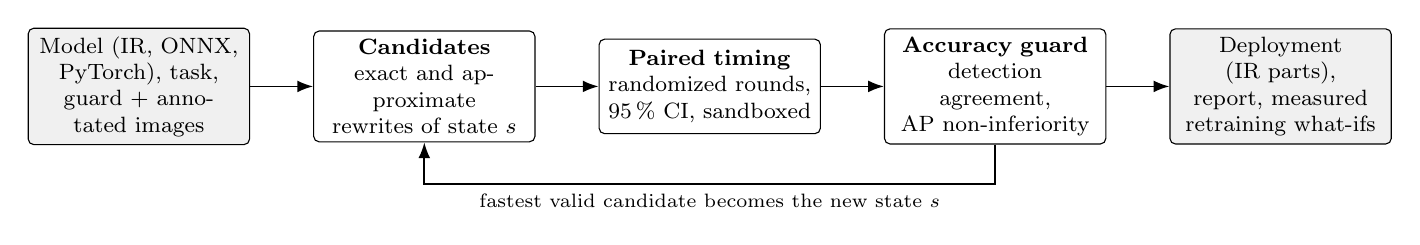
\begin{tikzpicture}[
  node distance=4mm and 8mm,
  box/.style={draw, rounded corners=2pt, align=center, font=\footnotesize, inner sep=3pt,
              minimum height=12mm, text width=26mm},
  io/.style={box, fill=black!6},
  arr/.style={-{Latex[length=2mm]}, semithick}]
\node[io] (in) {Model (IR, ONNX,\\PyTorch), task,\\guard + annotated images};
\node[box, right=of in] (cand) {\textbf{Candidates}\\exact and approximate\\rewrites of state $s$};
\node[box, right=of cand] (time) {\textbf{Paired timing}\\randomized rounds,\\95\,\% CI, sandboxed};
\node[box, right=of time] (guard) {\textbf{Accuracy guard}\\detection agreement,\\AP non-inferiority};
\node[io, right=of guard] (out) {Deployment (IR parts),\\report, measured\\retraining what-ifs};
\draw[arr] (in) -- (cand);
\draw[arr] (cand) -- (time);
\draw[arr] (time) -- (guard);
\draw[arr] (guard) -- (out);
\draw[arr] (guard.south) -- ++(0,-5mm) -| node[pos=0.25, below, font=\scriptsize] {fastest valid candidate becomes the new state $s$} (cand.south);
\end{tikzpicture}
\caption{The \tool{} optimization loop. Every candidate is timed against the current state in the same sandboxed process, and checked against the CPU FP32 original before it is accepted. The loop stops when no candidate is accepted.}
\label{fig:overview}
\end{figure*}

\subsection{Premise: latency does not depend on dense weight values}
\label{sec:premise}

We time each model with its trained weights and with variants of its inputs and weights, in paired adaptive rounds (Table~\ref{tab:premise}). Without an in-graph selection, real images, all-zero inputs and random dense weights change latency by at most 1.4\,\%. Two exceptions matter:
\begin{itemize}
\item \textbf{Data-dependent operations.} YOLO26 selects boxes with an in-graph \texttt{TopK}: on real images and with random weights, YOLO26-N runs 4.6 to 5.6\,\% faster than on the fixed noise input. Without this selection, which \tool{} moves to the CPU, the premise holds again. D-FINE samples deformable attention~\cite{zhu2021deformable} at data-dependent locations, with little effect (0.7\,\% at most).
\item \textbf{Weight sparsity.} The NPU skips zero weights: ResNet-50 is 26 and 35\,\% faster with 50 and 90\,\% of its weights at zero, and its mixed-INT8 deployment 24 and 39\,\%. Only 1.6 to 3.6\,\% of the INT8 weights of our deployments are zero, and setting them to one changes nothing measurable. Zero activations are not skipped: with dense non-positive weights and negative biases, every ReLU outputs zero, yet neither ResNet-50 ($+0.9 \pm 0.5\,\%$) nor YOLO26-N with ReLU ($-0.2 \pm 1.9\,\%$) gets faster.
\end{itemize}

\begin{table}[t]
\caption{Latency change of a variant relative to the trained model on a fixed noise input, in \% with 95\,\% CIs (NPU, two tiles; CNNs at 640~px, the mixed-INT8 ResNet-50 at 224~px). ``Head'': YOLO26-N without its final selection.}
\label{tab:premise}
\centering
\scriptsize
\setlength{\tabcolsep}{1.5pt}
\begin{tabular}{@{}lccccc@{}}
\toprule
& Real & Zero & Random & 50\,\% zero & 90\,\% zero \\
Model & images & input & weights & weights & weights \\
\midrule
ResNet-50 & $-0.2{\pm}0.2$ & $+0.3{\pm}0.4$ & $+0.1{\pm}0.4$ & $\mathbf{-25.9}{\pm}0.4$ & $\mathbf{-35.1}{\pm}0.3$ \\
ResNet-50 mixed & $+1.4{\pm}0.7$ & $+0.9{\pm}3.1$ & $-0.4{\pm}0.5$ & $\mathbf{-23.5}{\pm}0.7$ & $\mathbf{-39.1}{\pm}0.5$ \\
MobileNetV2 & $+1.0{\pm}1.3$ & $+1.0{\pm}1.6$ & $+1.0{\pm}0.8$ & $-1.9{\pm}0.9$ & $-4.6{\pm}1.3$ \\
YOLO26-N FP16 & $\mathbf{-5.6}{\pm}0.5$ & $0.0{\pm}0.5$ & $\mathbf{-4.6}{\pm}0.2$ & $-6.0{\pm}0.3$ & $-8.6{\pm}0.2$ \\
YOLO26-N INT8 & $\mathbf{-5.6}{\pm}0.3$ & $+0.1{\pm}0.3$ & $\mathbf{-3.3}{\pm}0.3$ & $-6.1{\pm}0.2$ & $-6.6{\pm}0.5$ \\
YOLO26-N head & $-0.4{\pm}0.7$ & $-0.9{\pm}0.9$ & $-0.9{\pm}0.8$ & $-1.6{\pm}0.7$ & $-6.0{\pm}0.7$ \\
D-FINE-N & $+0.5{\pm}0.3$ & $+0.7{\pm}0.3$ & $+0.1{\pm}0.3$ & $-2.2{\pm}0.1$ & $-2.5{\pm}0.2$ \\
\bottomrule
\end{tabular}
\end{table}

This premise has two consequences. \tool{} can time a rewrite before training it, for example SiLU replaced by ReLU in a model whose weights are not yet retrained: the sparsity of the retrained activations will not change its latency. Unstructured pruning becomes a rewrite whose speedup can be measured in advance, in FP16 as in INT8. Every variant is timed on the same fixed input (uniform noise in the input range), so that comparisons are paired; only YOLO26's in-graph selection runs at a different speed on real images.

\subsection{Measured profiler}
\label{sec:profiler}

\textbf{Regions.} The profiler attributes latency to \emph{regions}, sets of runtime operations that come from the same source module (PyTorch module paths, or ONNX node scopes), truncated at a depth chosen to give a target number of regions. It also attributes latency to operation types.

\textbf{Bypassing a region.} To bypass a region, \tool{} removes its operations and reconnects every tensor the region hands to the rest of the graph to the one tensor it receives with the same shape and type. The rewrite is refused when this mapping is ambiguous, or when it would create a cycle, which happens for a region that is not contiguous. Outputs that are no longer real are converted so that the graph stays valid. The saving of the bypassed graph is the latency of that region in context, fusions with its neighbors included. This saving is marginal: the compiler re-optimizes every bypassed graph, so the savings of the regions do not add up to the latency (O4). The profiler uses them to rank interventions, not to split the latency.

\textbf{Paired, randomized, adaptive rounds.} All variants and the reference are compiled in a single child process. Each round times every variant (30 to 40 inferences each) in a freshly shuffled order. A variant's saving is the mean of its per-round differences with the reference, with a 95\,\% confidence interval (normal approximation, $\pm 1.96$ standard errors). Pairing cancels the drift of the machine. Rounds continue until every half-width is at most $\max(0.02\ms, 0.5\,\%)$ of the latency, up to 40 rounds. A saving is \emph{significant} when its lower bound is positive.

\subsection{Task-level accuracy guard}
\label{sec:guard}

The reference is always the original model on the CPU in FP32. The guard has two levels.

\textbf{Agreement.} Both deployments run on 30 guard images. The agreement is the F1 score of matching their detections: same class, IoU $\geq 0.7$, confidence $\geq 0.3$. Without annotations, a state is exact when its agreement is at least $\tau = 0.95$. For a classifier, the agreement is the share of images with the same top-1 class; for any other model, it is $1 -$ the relative L2 error of the worst output. Table~\ref{tab:guard} calibrates the threshold on the two-tile faults of O5: any $\tau$ between 0.87 and 0.97 flags every fault that costs more than 0.5~AP, and we take 0.95. The calibration uses the evaluated models themselves, but $\tau$ only decides without annotations: none of the results of Section~\ref{sec:eval-optimizer} depends on it.

\begin{table}[t]
\caption{Agreement with CPU FP32 on 30 images, against the real AP loss of the two-tile mode (full val2017).}
\label{tab:guard}
\centering
\footnotesize
\begin{tabular}{@{}lccc@{}}
\toprule
& AP loss & \multicolumn{2}{c}{Agreement} \\
\cmidrule(l){3-4}
Model & (2 tiles) & 2 tiles & 1 tile \\
\midrule
RF-DETR-N & 0.0 & 0.990 & 0.990 \\
D-FINE-N & $-0.2$ & 0.919 & 0.994 \\
DEIMv2-N & $-0.9$ & 0.862 & 0.975 \\
RT-DETRv2-R18 & $-3.8$ & 0.729 & 0.990 \\
YOLO26-N & $-4.6$ & 0.842 & 0.989 \\
\bottomrule
\end{tabular}
\end{table}

\textbf{AP non-inferiority.} Agreement is only a proxy, and it errs both ways. The two-tile YOLO26-N reached 0.966 on one set of 30 images while losing more than 4~AP; D-FINE-N reaches only 0.923 while losing 0.2~AP. When annotations are given, the AP therefore decides: \tool{} evaluates it on $K = 20$ interleaved folds of 50 images, for the candidate and for the CPU FP32 reference. With the per-fold differences $d_k$, it accepts the candidate when a one-sided paired $t$ test rejects a loss larger than the budget $B$~\cite{wellek2010testing}:
\begin{equation}
\bar d - t_{0.95,\,K-1}\, \frac{s_d}{\sqrt{K}} \;\geq\; -B .
\label{eq:noninf}
\end{equation}
We use $B = 0.5$~AP. For a classifier, the same test applies to top-1 accuracy on a labeled set, with the same budget in accuracy points. This test decides whether the original deployment, a repair or an approximation counts as exact; with annotations, agreement only pre-filters the candidates.

\textbf{Test power.} Table~\ref{tab:ablation} shows what the test and its number of folds prevent. With 20 folds, the margins of approximate candidates close to the budget are 0.16 to 0.45 points on the seven detectors, and D-FINE-N's original deployment ($-0.18$, lower bound $-0.44$) is now exact. Top-1 on 2\,000 ImageNetV2 images is noisier, with margins of 0.37 to 0.92 points: a classifier mix passes only when it shows almost no loss.

\textbf{Confirmation.} The optimizer tests several candidates on the same decision images, and the mixed-precision search tests growing mixes until one passes. Keeping the first success among noisy tests favors an underestimated loss. An approximation that passes Eq.~(\ref{eq:noninf}) must therefore pass it again on held-out images, disjoint from all others, before it is accepted. A mix that fails ends the search: trying the next one would select on the held-out images too. Exact rewrites and repairs are not confirmed, since they are not meant to change the function. The confirmation removes the selection bias at a cost in power, since a candidate must pass two tests. On 1\,000 held-out COCO images, the margins are 0.19 to 0.28 points, and a candidate that truly loses 0.25 points fails the confirmation in 30 to 60\,\% of the cases. On 2\,000 ImageNetV2 images, the margins (0.67 to 0.98 points) exceed the budget: a mix without any loss passes the confirmation in only 20 to 30\,\% of the cases.

\begin{table}[t]
\caption{What the design choices prevent: the decision taken without each of them, on our models.}
\label{tab:ablation}
\centering
\footnotesize
\setlength{\tabcolsep}{3pt}
\begin{tabular}{@{}>{\raggedright\arraybackslash}p{0.31\columnwidth}>{\raggedright\arraybackslash}p{0.66\columnwidth}@{}}
\toprule
Without & Outcome \\
\midrule
agreement (max.\ output error instead) & RF-DETR-N (exact) is flagged, YOLO26-N ($-4.6$~AP) passes \\
the test (point estimate, 200 images) & a YOLO26-N mix within 0.3 points passes, then loses 0.9 on the report images; the test rejects it ($-0.37$, bound $-1.2$) \\
the confirmation & ResNet-50's mix ($-0.00$, bound $-0.49$) is kept and loses 0.64 on the report images; held-out images reject it ($-0.90$, bound $-1.88$) \\
20 folds (10 folds of 50 images) & 15\ms{} paid to repair D-FINE-N's $-0.25$ (bound $-0.64$); with 20, its original is exact ($-0.18$, bound $-0.44$) \\
the \emph{rest} group & D-FINE-N still loses 3.1~AP with 18 of 20 groups in float; \emph{rest} alone recovers 2.85 \\
approximate repairs, mixed precision on an inexact state & RT-DETRv2 takes the one-tile decoder (71.0\ms{}) instead of INT8 (40.6), which the confirmation later rejects \\
\bottomrule
\end{tabular}
\end{table}

\subsection{Optimizer}
\label{sec:optimizer}

\textbf{State.} The optimizer searches over deployment states $s = (\text{graph}, \text{compile options}, \text{placement})$. The placement either runs the whole graph on the NPU, or cuts it into two IR parts, each with its own device and options.

\textbf{Target.} The network stays on the NPU: the point of an NPU is to leave the CPU and the iGPU free, at low power. Only a \emph{light selection tail} may move to the CPU. This tail is the first \texttt{TopK} or NMS and everything that depends on it, provided it has no convolution or matrix product; this is the host post-processing every deployment performs. Moving heavier parts, such as a DETR decoder, to the iGPU or the CPU is an explicit option that we use only as a reference point (Section~\ref{sec:eval-offload}).

\textbf{Candidates.} Table~\ref{tab:catalog} lists the rewrites, in three tiers:
\begin{itemize}
\item \emph{exact} rewrites do not change the function;
\item \emph{approximate} rewrites change it on purpose and must keep AP within the budget;
\item \emph{retraining} rewrites are only timed on the final state, and reported with their measured latency.
\end{itemize}

\begin{table}[t]
\caption{Rewrite catalog.}
\label{tab:catalog}
\centering
\footnotesize
\begin{tabular}{@{}lp{0.68\columnwidth}@{}}
\toprule
Tier & Rewrites \\
\midrule
Exact & final selection on the host CPU; one or two tiles; DETR decoder compiled apart on one tile; depthwise as dense block-diagonal convolution \\
Approximate & INT8 post-training quantization (NNCF CNN and transformer schemes); latency-guided mixed precision \\
Retraining & SiLU/HardSwish/GELU $\to$ ReLU; LayerNorm $\to$ BatchNorm; 50\,\% and 75\,\% unstructured pruning \\
\bottomrule
\end{tabular}
\end{table}

\textbf{Greedy loop (Algorithm~\ref{alg:optimize}).} At each step, all candidates are timed against the current state in one paired session. They are then checked in decreasing order of saving. The first candidate that is significantly faster (lower bound above zero and saving above 1\,\%) and passes the guard is applied. Approximate candidates are always judged against the CPU FP32 original, never against the current state, so their errors do not accumulate. The loop stops when no candidate is accepted, and after five steps at most; no run needed more than two.

\textbf{Repairs.} An inexact state (O5) accepts any candidate that repairs it, even a slower one: correctness comes first. A rewrite of the exact tier that is faster and agrees better, without passing the guard, is also accepted. Approximate candidates can repair too; for instance, INT8 removes the two-tile fault of RT-DETRv2. On an inexact state, mixed precision is searched only when full INT8 keeps the mean loss within the budget and misses only its lower bound, since keeping groups in float could bring the fault back.

\begin{algorithm}[t]
\caption{Measured greedy optimization}
\label{alg:optimize}
\begin{algorithmic}[1]
\Require model $M$, task, guard images, annotated set, AP budget $B$
\State $s \gets (M,\ \text{default options},\ \text{whole graph on the NPU})$
\State $x \gets \textsc{Exact}(s)$ \Comment{Eq.~(\ref{eq:noninf}), else agreement $\ge \tau$}
\For{at most five steps}
  \State $C \gets \textsc{Candidates}(s)$
  \State time $s$ and $C$ in paired rounds: savings $\Delta_c \pm h_c$
  \State $s' \gets \bot$
  \For{$c \in C$ in decreasing order of $\Delta_c$}
    \State $f \gets \Delta_c - h_c > 0$ \textbf{and} $\Delta_c > 1\,\%$ \Comment{faster}
    \If{$x$ \textbf{and not} $f$}
      \State \textbf{continue} \Comment{an exact state only accepts gains}
    \EndIf
    \State $ok \gets \textsc{Exact}(c)$
    \If{$c$ approximate \textbf{and not} $ok$ \textbf{and} ($x$ \textbf{or} mean loss $\le B$)}
      \State $(ok, c) \gets \textsc{MixedPrecision}(s, c)$ \Comment{first mix that passes}
    \EndIf
    \If{$c$ approximate \textbf{and} $ok$}
      \State $ok \gets \textsc{Confirmed}(c)$ \Comment{held-out images}
    \EndIf
    \If{$ok$ \textbf{or} ($c$ exact-tier \textbf{and not} $x$ \textbf{and} $f$ \textbf{and} $c$ agrees better than $s$)}
      \State $s' \gets c$; \textbf{break}
    \EndIf
  \EndFor
  \If{$s' = \bot$}
    \State \textbf{break}
  \EndIf
  \State $s \gets s'$; $x \gets \textsc{Exact}(s)$
\EndFor
\State \Return $s$ and the measured latency of the retraining rewrites on $s$
\end{algorithmic}
\end{algorithm}

\textbf{Latency-guided mixed precision.} The search starts when full INT8 is significantly faster but outside the AP budget. It forms \emph{groups} of operations to keep in float:
\begin{itemize}
\item one group per module region that contains a convolution or a matrix product, with about ten groups in total;
\item one group, \emph{rest}, for every other quantized operation. Without it, quantizers on a DETR decoder's box arithmetic can never return to float (Section~\ref{sec:case-mixed}).
\end{itemize}
Each group is kept alone in float on top of full INT8, quantized with 64 calibration images. Its AP gain is measured on the annotated set, and its latency cost in a paired session against full INT8. Among the groups that cost more than a quarter of the INT8 saving, the most useful one that can be split is split into its sub-modules and measured again, up to three times. Groups are then ranked by AP gained per millisecond. Growing mixes are quantized with all 300 calibration images and \emph{verified as a whole}, for latency and with Eq.~(\ref{eq:noninf}). The search stops at the first mix that passes, which must then be confirmed, or when adding float groups removes the significant gain. We never assume that the latency of a mix is the sum of its groups' costs.

\subsection{Implementation}

\tool{} is a Python library and command-line tool (\texttt{optinpu profile}, \texttt{optinpu optimize}) built on OpenVINO and NNCF. Every compilation and inference runs in a child process watched for memory and time, whose whole process tree is killed on failure. On this NPU, the compiler reached 53 to 55\,GB of virtual memory on some graphs, and a lost device must become a rejected candidate rather than a crash of the tool. The optimized deployment is saved as IR parts with a JSON description (devices, compile options, applied changes) and a report. It can also be rebuilt from its list of changes: the seven rebuilt detector deployments reproduce their recorded AP exactly.

% =====================================================================================================
\section{Evaluation}

\subsection{Setup}

\textbf{Hardware and software.} We use an Intel Core Ultra~5 235U laptop (NPU 3720, driver 32.0.100.4778, 15.5\,GB of RAM) on mains power, with Windows~11 (Balanced power plan), OpenVINO 2026.4.1 and NNCF 3.4. A latency is the time of one synchronous batch-1 inference of the whole deployment, timed as in Section~\ref{sec:profiler}: all parts back to back, transfers and the CPU tail included, image decoding and resizing excluded.

\textbf{Models.} We use seven detectors, chosen to cover the architectural families that behave differently on the NPU:
\begin{itemize}
\item YOLO26-N and -S~\cite{jocher2026yolo26}: CNNs with an in-graph \texttt{TopK}, no NMS;
\item D-FINE-N and -S~\cite{peng2025dfine}, and DEIMv2-N~\cite{huang2025deimv2}: HGNetv2 backbones and deformable decoders;
\item RT-DETRv2-R18~\cite{lv2024rtdetrv2}: a ResNet backbone and a standard attention decoder;
\item RF-DETR-N~\cite{robinson2026rfdetr}: a DINOv2 ViT backbone~\cite{oquab2024dinov2}.
\end{itemize}
They are exported as FP16 IRs. To show that the approach is not specific to detection, we also optimize three ImageNet classifiers~\cite{russakovsky2015imagenet} at 224~px, with their torchvision weights: ResNet-50~\cite{he2016resnet}, MobileNetV2~\cite{sandler2018mobilenetv2} and EfficientNet-B0~\cite{tan2019efficientnet}. The profiler validation uses the same three CNNs at 640~px.

\textbf{Protocol.} All detectors were trained on COCO train2017, so every decision is taken on val2017 images disjoint from the reported ones: guard [4970, 5000), INT8 calibration [4500, 4800), AP budget [2500, 3500) in 20 folds of 50 images, and confirmation [3500, 4500), also in 20 folds. We report AP on val2017 [0, 2500), on which nothing is decided. The classifiers are judged on ImageNetV2~\cite{recht2019imagenetv2} (matched frequency, 10\,000 images), which none of them was trained on. We split one fixed shuffle of it into disjoint slices: guard [7300, 7600) (top-1 agreement), calibration [7000, 7300), top-1 budget [5000, 7000) in 10 folds of 200, confirmation [7600, 9600), also in 10 folds, and report [0, 5000). Unless noted, the latencies of a model's deployments come from one final paired session, timed against the original on the NPU in up to 60 rounds, with 95\,\% confidence intervals.
\subsection{Does measured profiling pick better interventions?}
\label{sec:eval-profiler}

\textbf{Ground truth.} On five models we apply 150 interventions: bypassing a region or an operation type, SiLU $\to$ ReLU, removing LayerNorms, and moving the final selection to the CPU. We measure each intervention's saving twice, in opposite orders, with up to 120 adaptive rounds. Run~1 is the ground truth; run~2 is an independent repetition.

\textbf{Predictors.} We compare four ways to predict these savings:
\begin{itemize}
\item \emph{vendor counters}: the durations of the removed operations, scaled to the latency;
\item an \emph{additive} model in the style of nn-Meter: each operation compiled alone on the NPU, minus the cost of a graph reduced to its inputs;
\item a \emph{learned} predictor: a ridge regression trained, for each model, on the run-1 savings of the four other models, from the two predictions above, the number of removed operations and the kind of intervention;
\item \emph{our measurement}: run~2, which shows how reproducible one measured run is and bounds what any predictor can reach.
\end{itemize}

\textbf{Metrics.} Over the 92 interventions that are significant in run~1, we report Spearman's $\rho$, the mean absolute error as a percentage of the latency, the overlap of the top three interventions, and the \emph{regret}: the share of the best saving lost by applying the predictor's first choice.

\begin{table}[t]
\caption{Predicting the saving of an intervention, against run~1: mean over five models (92 significant interventions out of 150).}
\label{tab:profiler}
\centering
\footnotesize
\begin{tabular}{@{}lcccc@{}}
\toprule
Predictor & $\rho$ & Error (\% lat.) & Top-3 & Regret \\
\midrule
Vendor counters (scaled) & $+0.36$ & 3.2 & 0.60 & 0.31 \\
Additive (isolated ops) & $+0.49$ & 9.5 & 0.67 & 0.60 \\
Learned (other models) & $+0.28$ & 3.8 & 0.53 & 0.21 \\
\textbf{Measured (run 2)} & $\mathbf{+0.84}$ & \textbf{0.8} & \textbf{0.87} & \textbf{0.00} \\
\bottomrule
\end{tabular}
\end{table}

Table~\ref{tab:profiler} gives the results. Run~2 never misses the best intervention of run~1: its regret is 0 on every model. The vendor counters have a regret of 0.63 on D-FINE-N and 0.78 on EfficientNet-B0. The additive model has a regret of 0.99 on YOLO26-N and 0.78 on ResNet-50; on YOLO26-N, both baselines even rank the interventions in the wrong order ($\rho = -0.04$ and $-0.10$). Fitting a predictor to measurements of this NPU does not help: the learned one ranks worse than both (regret 0.94 on D-FINE-N), and a gradient-boosted regressor does no better (regret 0.31). With five models its training data is small, but it would have to learn decisions the compiler takes on the whole graph (O4). This accuracy has a cost: one measured run of all the interventions of a model takes 1.8 to 12~minutes (36~minutes for the five models), against 2 to 4~s for the vendor counters and 0.6 to 2.3~minutes for the additive model. Summed over all operations of the four larger models, the counters give 123 to 297\ms{} and the additive model 72 to 260\ms{}, for real latencies of 17 to 31\ms{}.

\textbf{Limit.} On the smallest model (MobileNetV2, 7.0\ms{}), 21 of the 23 savings are significant but close to each other, and their fine order stays at the noise level even after 120 rounds: the repeated measurement ranks them less consistently ($\rho = +0.68$) than the vendor counters ($+0.74$), but still picks the best one (regret 0, against 0.12).

\subsection{Optimizing detectors for the NPU}
\label{sec:eval-optimizer}

Table~\ref{tab:results} reports the optimizer with the network on the NPU (Section~\ref{sec:optimizer}).

\begin{table*}[t]
\caption{Optimizer results, network on the NPU, with the confirmation (FP16 IRs; AP on val2017 [0, 2500), on which nothing was decided). Latencies from one paired session per model: ``before'' is the default two-tile compilation; ``after'' is before minus the paired saving, with its 95\,\% half-width.}
\label{tab:results}
\centering
\footnotesize
\begin{tabular}{@{}lll>{\raggedright\arraybackslash}p{0.30\textwidth}c@{}}
\toprule
Model & Before & After & Applied changes & AP: CPU FP32 / before / after \\
\midrule
YOLO26-N & 26.7\ms{} & \textbf{9.40 $\pm$ 0.09\ms{} (2.84$\times$)} & final selection on the CPU & 41.7 / 37.0 / 41.6 \\
YOLO26-S & 33.0\ms{}, device lost & \textbf{16.35 $\pm$ 0.16\ms{} (2.02$\times$)} & final selection on the CPU & 49.4 / --- / 49.4 \\
D-FINE-N & 26.0\ms{} & 26.0\ms{} (1.00$\times$) & none: the original is exact & 44.5 / 44.3 / 44.3 \\
D-FINE-S & 46.9\ms{} & 46.9\ms{} (1.00$\times$) & none: mixed INT8 not confirmed$^\ast$ & 50.2 / 50.1 / 50.1 \\
DEIMv2-N & 23.9\ms{} & 41.01 $\pm$ 0.03\ms{} (0.58$\times$) & repair: one tile (original AP $-0.44$, bound $-0.69$) & 45.0 / 44.0 / 44.9 \\
RT-DETRv2-R18 & 47.4\ms{} & 76.09 $\pm$ 0.08\ms{} (0.62$\times$) & repair: decoder on one tile; INT8 not confirmed$^\ast$ & 49.7 / 46.0 / 49.7 \\
RF-DETR-N & 83.3\ms{} & 81.82 $\pm$ 0.06\ms{} (1.02$\times$) & INT8, transformer scheme & 50.0 / 50.0 / 49.7 \\
\bottomrule
\multicolumn{5}{@{}l@{}}{\scriptsize $^\ast$Without the confirmation: D-FINE-S 42.9\ms{} (1.08$\times$, AP 49.9) with 7 of 19 groups in float; RT-DETRv2 40.6\ms{} (1.17$\times$, AP 49.6) with INT8 in the transformer scheme.}
\end{tabular}
\end{table*}

\textbf{YOLO26.} The optimizer moves 16 operations, the final selection, to the CPU. This makes YOLO26-N 2.84$\times$ faster and YOLO26-S 2.02$\times$ faster on the NPU (YOLO26-N about 2.7$\times$ on real images, on which its in-graph selection runs 5.6\,\% faster, Table~\ref{tab:premise}). Exporting a detector without its final selection is a common deployment practice. The measurement adds that this tail costs two thirds of the latency (Section~\ref{sec:case}), and the guard shows that removing it also removes both two-tile faults: the silent loss of 4.6~AP of YOLO26-N, and the device hang of YOLO26-S. The tail compiled alone on two tiles does not hang, so the faults arise when the compiler combines the selection with the rest of the graph. Mixed INT8 would then save up to 2.7\ms{} more on YOLO26-S, but every mix loses about 0.5~AP (lower bounds $-0.73$ to $-0.89$) and is rejected, as on YOLO26-N.

\textbf{DETR family.} Without leaving the NPU, the DETRs mostly need repairs, and the guard decides what they may cost:
\begin{itemize}
\item \emph{RT-DETRv2} loses 3.7~AP in two-tile mode on the report images. INT8 with the transformer scheme repairs it and is faster (40.6\ms{}), within 0.1~AP of the CPU on the report images, but it loses 0.47~AP on the held-out images (bound $-0.72$) and is not confirmed. The optimizer then takes an exact repair, the decoder compiled apart on one tile: 76.1\ms{}, with the AP of the CPU (Section~\ref{sec:case-repair}).
\item \emph{DEIMv2-N} loses 0.44~AP on the decision images (lower bound $-0.69$), and 1.0 on the report images. Neither INT8 scheme stays within the budget ($-22.5$ and $-1.2$~AP), and the decoder alone on one tile is slower than the whole graph on one tile. The cheapest exact deployment therefore runs on one tile: 41.2\ms{} instead of 24.0. With a budget of one point, the original would be kept; the report gives both.
\item \emph{D-FINE-N} loses only 0.18~AP: the original is exact, and nothing else is both faster and within the budget. Full INT8 saves only 0.3\ms{} and costs 5.9~AP, most of it in the backbone.
\item \emph{D-FINE-S} and \emph{RF-DETR-N} are exact on the NPU. Full INT8 costs D-FINE-S 6.0~AP; keeping 7 of 19 groups in float, the \emph{rest} group included, brings it within the budget ($-0.13$, bound $-0.36$), and this mix is even 1.3\ms{} faster than full INT8. The held-out images do not confirm it ($-0.25$, bound $-0.52$), and the original is kept; on the report images, the mix loses 0.27~AP, within the budget but not certified. RF-DETR-N gains only 2\,\%, with INT8 in the transformer scheme, confirmed ($-0.22$, bound $-0.41$); it loses 0.27~AP on the report images.
\end{itemize}
On the NPU alone, none of them beats its best placement of Table~\ref{tab:m0}.


\subsection{Beyond detection: image classifiers}
\label{sec:eval-classifiers}

The same optimizer runs on classifiers, with the top-1 agreement as guard and top-1 accuracy as the judged metric (Table~\ref{tab:classifiers}). On the report slice, CPU FP32 top-1 is 11 to 13 points below each model's ImageNet accuracy, as expected~\cite{recht2019imagenetv2}. The compiler is exact on all three (within 0.15 points of the CPU), so only INT8 can make them faster. On ResNet-50, full INT8 is 1.62$\times$ faster but loses 0.30 points (bound $-0.90$); keeping 5 of 20 groups in float passes the test ($-0.00$, bound $-0.49$) and keeps 1.43$\times$. On MobileNetV2, full INT8 saves 19\,\% and loses 0.35 points; four groups in float pass ($+0.05$, bound $-0.47$) at almost no cost. On EfficientNet-B0, full INT8 saves only 6\,\% and loses 1.25 points, no group recovers more than 0.2 points when kept in float, and the original is kept. Depthwise convolutions rewritten as dense ones are slower on both mobile networks.

Neither mix is confirmed, and the original is kept on all three classifiers. ResNet-50's mix loses 0.90 points on the held-out images (bound $-1.88$) and 0.64 on the report images: the search had tested five growing mixes on the same images and kept the first that passed, after four with point estimates of $-0.05$ to $-0.30$, which favors an underestimated loss. MobileNetV2's mix gains 0.15 points on the held-out images, but its bound ($-0.53$) misses the budget: 2\,000 images cannot certify a loss below half a point. An earlier run without the confirmation had kept a mix on both: 1.60$\times$ and 1.22$\times$, with $-0.64$ and $+0.1$ points on the report images.

\begin{table}[t]
\caption{Classifiers, network on the NPU (224~px), in the optimizer's run with the confirmation: the mix that passes Eq.~(\ref{eq:noninf}), and its top-1 change against CPU FP32 in points (95\,\% lower bound) on the decision and held-out images. The original is kept on all three; on ImageNetV2 [0, 5000), it is within 0.15 points of CPU FP32.}
\label{tab:classifiers}
\centering
\footnotesize
\setlength{\tabcolsep}{3pt}
\begin{tabular}{@{}lcccc@{}}
\toprule
& Before & Mix & \multicolumn{2}{c}{Top-1 change (bound)} \\
\cmidrule(l){4-5}
Model & (ms) & (ms) & decision & held-out \\
\midrule
ResNet-50 & 4.52 & 3.16 (1.43$\times$) & $-0.00$ ($-0.49$) & $-0.90$ ($-1.88$) \\
MobileNetV2 & 1.40 & 1.14 (1.23$\times$) & $+0.05$ ($-0.47$) & $+0.15$ ($-0.53$) \\
EfficientNet-B0 & 2.75 & none & --- & --- \\
\bottomrule
\end{tabular}
\end{table}

\subsection{Against NNCF's accuracy-aware quantization}
\label{sec:eval-nncf}

NNCF's \texttt{quantize\_with\_accuracy\_control}~\cite{kozlov2020nncf} is the closest existing tool: starting from full INT8, it returns to float, one at a time, the quantizers that hurt the metric most, until the drop on a validation set is at most a given value. We give it what \tool{}'s search had: the same graph (for YOLO26, the network without its selection), calibration images, decision images and budget (0.5 point); it validates on the CPU. Table~\ref{tab:nncf} compares the results on the NPU.

\begin{table}[t]
\caption{NNCF's accuracy-aware quantization against \tool{}, on the NPU: search time, latency (one paired session) and metric change against CPU FP32 on the report images, in points.}
\label{tab:nncf}
\centering
\footnotesize
\setlength{\tabcolsep}{3.5pt}
\begin{tabular}{@{}lccccc@{}}
\toprule
& \multicolumn{3}{c}{NNCF} & \multicolumn{2}{c}{\tool{}} \\
\cmidrule(lr){2-4}\cmidrule(l){5-6}
Model & Search & ms & $\Delta$ & ms & $\Delta$ \\
\midrule
ResNet-50 & 2 min & 1.99 & $-0.4$ & 3.81$^\ast$ & $0.0$ \\
MobileNetV2 & 1 min & 0.79 & $-0.2$ & 1.03$^\ast$ & $0.0$ \\
EfficientNet-B0 & 25 min & 2.60 & $\mathbf{-1.5}$ & 2.77 & $0.0$ \\
YOLO26-N & 82 min & 8.51 & $\mathbf{-18.2}$ & 9.20 & $-0.1$ \\
YOLO26-S & 146 min & 13.69 & $-0.3$ & 16.27 & $0.0$ \\
D-FINE-S & $>$6~h & \multicolumn{2}{c}{budget not reached} & 46.9$^\ast$ & $-0.1$ \\
\bottomrule
\multicolumn{6}{@{}l@{}}{\scriptsize $^\ast$The original: Eq.~(\ref{eq:noninf}) alone accepts a mix (2.40\ms{} and $-0.6$; 0.81 and 0.0;}\\
\multicolumn{6}{@{}l@{}}{\scriptsize 42.9 and $-0.3$), which the confirmation rejects.}
\end{tabular}
\end{table}

None of NNCF's models passes Eq.~(\ref{eq:noninf}) on the decision images: a point estimate accepts losses that 1\,000 images cannot certify. Where its model stays within the budget on the report images (ResNet-50, MobileNetV2, YOLO26-S), it is faster than \tool{}'s deployment, which keeps the original classifiers once the confirmation has rejected their mixes: 1.99 against 3.81\ms{} on ResNet-50, 0.79 against 1.03 on MobileNetV2, and 13.69 against 16.27 on YOLO26-S. Our test is the more conservative: it refuses losses it cannot certify, and here this costs three models their INT8 gain. Validating on the CPU, however, misses the NPU: EfficientNet-B0 loses 1.5 points and YOLO26-N 18.2~AP on the NPU, although both stayed within the budget on the CPU. The INT8 network of YOLO26-N without its selection is wrong on the NPU only, a fault that no check on the CPU can see. On D-FINE-S, NNCF had not reached the budget after 6~h: after 38 iterations, it still lost 3.4~AP, spread over the decoder's box arithmetic (Section~\ref{sec:case-mixed}).

\subsection{Reference point: the iGPU, optimized the same way}
\label{sec:eval-igpu}

Table~\ref{tab:m0} compares the NPU with the original model on the iGPU. For a fair comparison, we also run \tool{} for the iGPU, with the same rewrites, budget, images and confirmation, and time both optimized deployments in the final session (Table~\ref{tab:igpu}). INT8 works far better on the iGPU: it is confirmed on four of the seven detectors (1.28 to 1.78$\times$ faster than the original on the iGPU), against one on the NPU (1.02$\times$). D-FINE-N and -S run 1.36 and 1.74$\times$ faster with INT8 in the transformer scheme and their backbone in FP16, while on the NPU this scheme makes D-FINE-S slower (53.0 against 47.1\ms{}). RT-DETRv2's INT8 is rejected by the confirmation on both devices ($-0.47$ and $-0.58$~AP on the held-out images). Optimized this way, the iGPU is faster than the NPU on seven of the ten models, by 1.3 to 4.5$\times$; the NPU stays faster on YOLO26-S (16.4 against 20.2\ms{}) and ResNet-50 (3.75 against 4.33\ms{}). MobileNetV2 is a tie: its latency on the NPU varied from 1.1 to 1.6\ms{} between sessions, more than its difference with the iGPU.

\begin{table}[t]
\caption{NPU against iGPU, both optimized by \tool{} with the confirmation and timed in one paired session per model (95\,\% half-widths 0.03 to 0.18\ms{}): latency in ms, and in parentheses the metric change against CPU FP32 on the report images, in points. ---: nothing applied.}
\label{tab:igpu}
\centering
\footnotesize
\setlength{\tabcolsep}{2.5pt}
\begin{tabular}{@{}lcccl@{}}
\toprule
& NPU & \multicolumn{3}{c}{iGPU} \\
\cmidrule(lr){2-2}\cmidrule(l){3-5}
Model & optimized & original & optimized & changes \\
\midrule
YOLO26-N & 9.40 ($-0.1$) & 11.19 & \textbf{6.29} ($-0.5$) & mixed INT8 \\
YOLO26-S & \textbf{16.35} ($0.0$) & 23.53 & 20.21 ($0.0$) & selection on CPU \\
D-FINE-N & 25.97 ($-0.2$) & 17.55 & \textbf{13.86} ($-0.1$) & INT8$^\ast$ \\
D-FINE-S & 46.93 ($-0.1$) & 43.02 & \textbf{25.16} ($-0.1$) & INT8$^\ast$ \\
DEIMv2-N & 41.01$^\dagger$ ($-0.1$) & \textbf{17.14} & --- & \\
RT-DETRv2-R18 & 76.09$^\dagger$ ($0.0$) & \textbf{47.58} & --- & \\
RF-DETR-N & 81.82 ($-0.3$) & 23.39 & \textbf{18.16} ($-0.3$) & INT8$^\ddagger$ \\
ResNet-50 & \textbf{3.75} ($0.0$) & 4.33 & --- & \\
MobileNetV2 & 1.59 ($0.0$) & \textbf{1.29} & --- & \\
EfficientNet-B0 & 2.81 ($0.0$) & \textbf{2.10} & --- & \\
\bottomrule
\multicolumn{5}{@{}l@{}}{\scriptsize $^\ast$transformer scheme, backbone in FP16. $^\ddagger$transformer scheme. $^\dagger$repaired.}
\end{tabular}
\end{table}

\subsection{Reference point: offloading the decoder}
\label{sec:eval-offload}

When the decoder may leave the NPU, the optimizer moves it to the iGPU on every DETR, 1.4 to 2.1$\times$ faster than the original on the NPU in its own run (Table~\ref{tab:offload}); there, it matched or beat the fastest placement of Table~\ref{tab:m0} on D-FINE-N, D-FINE-S and RT-DETRv2. Hybrid latencies are less stable than the others: timed again in the final session, the same deployments ran from 4\,\% faster to 24\,\% slower, while the originals on the NPU stayed within 1.5\,\% of their earlier latency. In that session, the hybrid deployment beats the original on the iGPU on D-FINE-S, DEIMv2-N and RT-DETRv2, ties on D-FINE-N and loses on RF-DETR-N; the optimized iGPU deployment is faster on D-FINE-N, D-FINE-S and RF-DETR-N. Three hybrid deployments also rely on approximations accepted without the confirmation, which rejected RT-DETRv2's INT8 on both devices. This is why \tool{} keeps the network on the NPU by default: offloading competes with other devices rather than optimizing for the NPU.

\begin{table}[t]
\caption{With the decoder allowed on the iGPU: \tool{}'s NPU+iGPU deployment in its own run and in the final session ($\pm$ 95\,\% half-width), its AP on val2017 [0, 2500), and the iGPU alone in the final session (original / optimized), in ms.}
\label{tab:offload}
\centering
\footnotesize
\setlength{\tabcolsep}{3pt}
\begin{tabular}{@{}lcccc@{}}
\toprule
& \multicolumn{2}{c}{NPU+iGPU} & AP CPU & iGPU \\
\cmidrule(lr){2-3}
Model & own run & final & / after & orig.\ / opt. \\
\midrule
D-FINE-N & 15.2 & 17.5 $\pm$ 0.5 & 44.5 / 44.4 & 17.6 / 13.9 \\
D-FINE-S & 30.3$^\ddagger$ & 35.0 $\pm$ 0.5 & 50.2 / 50.0 & 43.0 / 25.2 \\
DEIMv2-N & 16.6 & 16.0 $\pm$ 0.6 & 45.0 / 44.9 & 17.1 / --- \\
RT-DETRv2-R18 & 26.1$^{\ast\dagger}$ & 32.3 $\pm$ 0.3 & 49.7 / 49.6 & 47.6 / --- \\
RF-DETR-N & 40.1$^\dagger$ & 39.3 $\pm$ 0.4 & 50.0 / 49.7 & 23.4 / 18.2 \\
\bottomrule
\multicolumn{5}{@{}l@{}}{\scriptsize $^\ast$cut at the end of the encoder. $^\dagger$+ INT8 (transformer scheme). $^\ddagger$+ mixed INT8;}\\
\multicolumn{5}{@{}l@{}}{\scriptsize approximations accepted by Eq.~(\ref{eq:noninf}) alone, without the confirmation.}
\end{tabular}
\end{table}

\subsection{Energy per inference}
\label{sec:energy}

Windows exposes the RAPL energy counters of the whole package (CPU cores, iGPU, NPU and the rest of the SoC); the NPU has no counter of its own. We measure the package power during three 20\,s windows of back-to-back inferences, each after 4\,s at idle, with the display allowed to turn off (Fig.~\ref{fig:power}): 5.1 to 9.7\,W on the NPU, 7.2 to 9.3\,W with the decoder on the iGPU, 15.6 to 19.7\,W on the iGPU and 21.4 to 23.6\,W on the CPU, against 2.5 to 3.1\,W at idle. Multiplied by the latency, it gives the energy of one inference. On nine of the ten models, the NPU deployment uses 1.2 to 2.3$\times$ less energy than the iGPU deployment, even where the iGPU is faster, and the CPU 3.9 to 17$\times$ more. The exception is RF-DETR-N, whose optimized iGPU deployment is 4.5$\times$ faster and uses 1.3$\times$ less energy. On RF-DETR-N, and on RT-DETRv2 and DEIMv2-N, whose NPU deployments are slow repairs, the NPU+iGPU deployment uses the least energy. Counting only the power above idle, which is noisier, the NPU uses 1.3 to 3.5$\times$ less energy than the iGPU on all ten models. \texttt{NPU\_TURBO} changes the package power by $-0.2$ to $+0.4$\,W and the energy per inference by $-4$ to $+5\,\%$: its speedup costs no measurable energy. A first campaign, with 8\,s windows and the display on (7 to 10\,W at idle), gave higher energies and the same ranking, except on DEIMv2-N, whose one-tile deployment then used more energy than the iGPU.

\begin{figure}[t]
\centering
\definecolor{cnpu}{HTML}{2A78D6}
\definecolor{cnpugpu}{HTML}{EB6834}
\definecolor{cgpu}{HTML}{1BAF7A}
\definecolor{ccpu}{HTML}{EDA100}

\begin{tikzpicture}
\begin{axis}[scale only axis, width=0.72\columnwidth, height=3.6cm, xmin=0, xmax=25, ymin=0.4, ymax=10.6, xtick pos=bottom, xtick={0,5,...,25},
  ytick={1,...,10}, yticklabels={EfficientNet-B0,MobileNetV2,ResNet-50,RF-DETR-N,RT-DETRv2-R18,DEIMv2-N,D-FINE-S,D-FINE-N,YOLO26-S,YOLO26-N}, xlabel={Package power while inferring (W)},
  tick label style={font=\scriptsize}, label style={font=\footnotesize}, axis line style={black!60},
  tick style={black!60}, ytick style={draw=none}, xmajorgrids, major grid style={black!12},
  legend style={font=\scriptsize, draw=none, fill=none, at={(0.5,1.02)}, anchor=south, legend columns=4,
  /tikz/every even column/.append style={column sep=6pt}}, legend cell align=left]
\addplot[black!25, line width=0.8pt, forget plot] coordinates {(7.31,10) (21.8,10)};
\addplot[black!25, line width=0.8pt, forget plot] coordinates {(8.61,9) (21.5,9)};
\addplot[black!25, line width=0.8pt, forget plot] coordinates {(5.87,8) (22,8)};
\addplot[black!25, line width=0.8pt, forget plot] coordinates {(6.53,7) (21.6,7)};
\addplot[black!25, line width=0.8pt, forget plot] coordinates {(5.13,6) (23.6,6)};
\addplot[black!25, line width=0.8pt, forget plot] coordinates {(6.26,5) (22.4,5)};
\addplot[black!25, line width=0.8pt, forget plot] coordinates {(5.37,4) (22.7,4)};
\addplot[black!25, line width=0.8pt, forget plot] coordinates {(9.13,3) (21.4,3)};
\addplot[black!25, line width=0.8pt, forget plot] coordinates {(9.65,2) (22,2)};
\addplot[black!25, line width=0.8pt, forget plot] coordinates {(7.27,1) (21.6,1)};
\addplot[only marks, mark=*, mark size=2.2pt, color=cnpu, mark options={draw=white, line width=0.3pt}] coordinates {(7.31,10) (8.61,9) (5.87,8) (6.53,7) (5.13,6) (6.26,5) (5.37,4) (9.13,3) (9.65,2) (7.27,1)};
\addlegendentry{NPU}
\addplot[only marks, mark=diamond*, mark size=2.2pt, color=cnpugpu, mark options={draw=white, line width=0.3pt}] coordinates {(9.24,8) (9.1,7) (9.3,6) (9.09,5) (7.19,4)};
\addlegendentry{NPU+iGPU}
\addplot[only marks, mark=square*, mark size=2.2pt, color=cgpu, mark options={draw=white, line width=0.3pt}] coordinates {(16.8,10) (17.1,9) (15.6,8) (16.1,7) (15.8,6) (17.5,5) (18.7,4) (19.7,3) (16.1,2) (19.5,1)};
\addlegendentry{iGPU}
\addplot[only marks, mark=triangle*, mark size=2.2pt, color=ccpu, mark options={draw=white, line width=0.3pt}] coordinates {(21.8,10) (21.5,9) (22,8) (21.6,7) (23.6,6) (22.4,5) (22.7,4) (21.4,3) (22,2) (21.6,1)};
\addlegendentry{CPU}
\end{axis}
\end{tikzpicture}

\caption{Package power while inferring back to back: \tool{}'s NPU deployment (Tables~\ref{tab:results} and~\ref{tab:classifiers}), its NPU+iGPU deployment (Table~\ref{tab:offload}), the iGPU deployment (optimized when something was applied, Table~\ref{tab:igpu}), and the original on the CPU (FP32). At idle, the package draws 2.5 to 3.1\,W.}
\label{fig:power}
\end{figure}

\subsection{Case studies}
\label{sec:case}

\subsubsection{Where the time goes in YOLO26-N}
Bypassing the final selection (16 operations) saves 17.5\ms{}, two thirds of the 26.4\ms{} latency (Section~\ref{sec:eval-profiler}). The vendor counters point at the same operations, which run on the SHAVE cores (\texttt{Divide} 19.5\ms{}, \texttt{GatherElements} 15.4\ms{}, \texttt{TopK} 4.1\ms{}), but their durations overlap: over the 16 operations, they add up to 58.7\ms{}, twice the whole inference. Only the bypass measurement gives the real saving, which the selection-to-CPU rewrite then achieves (17.3\ms{}).

\subsubsection{Mixed precision is not additive}
\label{sec:case-mixed}
\textbf{The loss is concentrated.} On YOLO26-S, full INT8 loses 6.6~AP. Most of the loss sits in one attention block: keeping it in float recovers 4.5~AP for 0.04\ms{}.

\textbf{Latency is not additive.} On RF-DETR-N, whose backbone runs on the NPU, NNCF's CNN scheme loses 4.2~AP, and the optimizer refined the search down to the 12 DINOv2 layers. Keeping the \emph{whole} encoder stack in float costs 4.2\ms{}. Keeping a \emph{single} middle layer in float, between INT8 layers, costs 13 to 16\ms{}. Precision changes and the re-tiling between layers of different precisions cost more than the arithmetic. A cost model that sums per-layer costs would choose the single layer; measuring the whole mix avoids that mistake.

\textbf{Module groups miss operations.} On D-FINE-N, keeping 18 of 20 module groups in float still left a 3.1-point loss (Table~\ref{tab:ablation}). With every group in float, 64 quantizers remained, almost all on the decoder's box and reference-point arithmetic, which belongs to no module containing a convolution. The \emph{rest} group fixes this, and it becomes the most useful group of D-FINE-N: keeping it in float recovers 2.85~AP and even saves 0.47\ms{}.

\subsubsection{Repairing on the NPU}
\label{sec:case-repair}
On RT-DETRv2, the two-tile fault sits in the decoder's self-attention. Rewriting the attention in the IR changes nothing, because the compiler normalizes all its variants. Compiling the decoder apart on one tile, with the rest on two, repairs the model on the NPU (agreement 0.721 $\to$ 0.995), but costs 76.1\ms{} instead of 47.4: cutting the graph into two NPU inferences alone costs 8.9\ms{}, and one tile slows the decoder down by 19\ms{}. INT8 with the transformer scheme also removes the fault, because the compiler then partitions the attention differently, and it is faster than the original (40.6\ms{}). Two rules let the optimizer consider this repair (Section~\ref{sec:optimizer}): approximate candidates may repair an inexact state, and mixed precision may be searched on an inexact state when full INT8 keeps the mean loss within the budget. The INT8 repair passes Eq.~(\ref{eq:noninf}) on the decision images ($-0.11$, bound $-0.37$) and loses only 0.1~AP on the report images, but 0.47 on the held-out images (bound $-0.72$), and 0.58 on the iGPU: the confirmation rejects it, and the optimizer pays 35\ms{} for the repair it can certify.


\subsection{Retraining rewrites, measured before training}

Thanks to the premise, \tool{} reports the exact latency of rewrites that need retraining: SiLU $\to$ ReLU would make the optimized YOLO26-N 21\,\% faster (7.33\ms{}), YOLO26-S 17\,\% faster (13.4\ms{}) and EfficientNet-B0 35\,\% faster (1.79\ms{}); pruning 50\,\% or 75\,\% of the weights would make ResNet-50 18\,\% or 33\,\% faster (3.71 or 3.03\ms{}, from 4.52); on the five DETR-family models, the best of these rewrites brings only 3 to 9\,\%.
\tool{} does not retrain the model: it tells, before any training, which retraining is worth its cost. A gain of 17 to 35\,\% justifies fine-tuning YOLO26 or EfficientNet-B0 with ReLU; 3 to 9\,\% hardly justifies retraining a DETR.

% =====================================================================================================
\section{Discussion and Limitations}
\label{sec:limits}

\textbf{One NPU.} We measured a single NPU (3720), with a single driver and compiler version, and did not test \tool{} on another NPU. Its faults and costs may differ on other NPUs or change with a driver update; this is precisely why \tool{} measures instead of encoding rules. Porting it to another NPU supported by OpenVINO only requires a device name; another runtime would need new sandboxed jobs.

\textbf{Accuracy guard.} The guard relies on samples. Agreement on 30 images can miss AP losses (Section~\ref{sec:guard}), so AP decides when annotations exist; without them, an approximate rewrite must reach the agreement of an exact one, a conservative rule. The test averages AP over folds of 50 images; an image-level bootstrap of the AP would not assume normal fold differences. The confirmation removes the bias of keeping the first of several passing mixes, but costs power: it rejected three candidates whose mean loss stays within the budget (at most 0.47 points on the held-out images, and 0.27 on the report images where we measured it). More decision and held-out images would let such candidates pass; on the classifiers, 2\,000 held-out images are too few to confirm even a mix without any loss reliably. Every result uses $B = 0.5$~AP; a budget of one point would keep DEIMv2-N's original (24.0\ms{}) and accept YOLO26-S's mixes.

\textbf{Cost of the search.} The search applies one change at a time, so it can miss combinations that only pay off together. A whole run, final evaluation included, takes 12 to 24 minutes for a classifier and 35 minutes to 1~h~50 for a detector on our laptop. Re-running the optimizer reproduced its decisions up to the confirmation, with the same mixes on D-FINE-S and ResNet-50; only MobileNetV2, whose groups cost about 0.01\ms{} each, got a different mix. The optimizer explores one compile option (\texttt{NPU\_TILES}) and batch-1 latency. Measured on its deployments, other options change little: \texttt{NPU\_TURBO} saves up to 6.6\,\%, most on the smallest models, at no measurable energy cost (Section~\ref{sec:energy}), and the throughput hint and QDQ optimization nothing significant. With two inferences in flight, throughput rises by 2 to 9\,\% on the detectors, by 23 to 63\,\% on the classifiers, and doubles on the one-tile DEIMv2-N, whose two inferences then use a tile each; overlapping YOLO26's CPU tail with the next inference adds only 7 and 3\,\%. Beyond detectors and classifiers, other models can use the generic output-agreement task, without a metric test.

% =====================================================================================================
\section{Conclusion}

On the client NPU we studied, latency could not be predicted from FLOPs, vendor counters, per-operation costs or a regressor fitted to them, and the compiler was silently wrong. Two facts make a measurement-only approach practical: latency does not depend on dense weight values, and paired, randomized, adaptive rounds measure small savings reliably. \tool{} turns these facts into a profiler that picks the right intervention, an accuracy guard grounded in the task, and an optimizer that repairs and accelerates detectors without leaving the NPU. It repairs the four detectors that the compiler gets wrong and makes YOLO26-N and -S 2.84 and 2.02$\times$ faster (YOLO26-S stays ahead of the iGPU even when the iGPU is optimized the same way); checking accuracy on the CPU instead would have missed an 18-AP loss. Once approximations must hold on held-out images, INT8 helps little on this NPU: one DETR gains 1.02$\times$ and no classifier mix is confirmed, while the same optimizer confirms INT8 on four detectors on the iGPU. The NPU's advantage is then energy rather than speed: it uses less energy per inference than the iGPU on nine of the ten models. The measured what-ifs tell which retraining is worth its cost.

\section*{Acknowledgment}
The author used AI tools to help gather the references and write this paper, and reviewed all of its content.

\bibliographystyle{IEEEtran}
\bibliography{references}

\end{document}
